%
% The manuscript for P1EDA, short paper. 

\documentclass[11pt,letterpaper]{article}
\usepackage{naaclhlt2015}
\usepackage{times}
\usepackage{latexsym}
\usepackage{microtype}
\usepackage{amsmath,amssymb}
%\usepackage{microtype}
\usepackage{graphicx}
\usepackage{rotating}
\setlength\titlebox{6.5cm}    % Expanding the titlebox

\title{Multi-Level Alignments As an Abstraction Layer for Extendable,
  Multilingual Textual Entailment}


% \author{Author 1\\
% 	    XYZ Company\\
% 	    111 Anywhere Street\\
% 	    Mytown, NY 10000, USA\\
% 	    {\tt author1@xyz.org}
% 	  \And
% 	Author 2\\
%   	ABC University\\
%   	900 Main Street\\
%   	Ourcity, PQ, Canada A1A 1T2\\
%   {\tt author2@abc.ca}}

\date{}

\begin{document}
\maketitle
\begin{abstract}
  % SP: more motivation
  Textual Entailment technology has become more robust over the last
  years. Nevertheless, state-of-the-art models still rely on
  hand-crafted, incompatible data structures, which makes exchange of
  components very difficult in practice. In this paper, we introduce
  {\em multi-level alignments} as a very general representation to
  store information relevant for deciding entailment that can store
  many kinds of information, can be translated easily into features,
  and is applicable across languages. We demonstrate that a very
  simple open-source, pilot implementation of the approach already
  competes with much more complex state-of-the-art open-source TE
  engines across three languages.
\end{abstract}

\section{Introduction}
A key challenge of Natural Language Processing is to determine what
conclusions can be drawn from a natural language text, a task known as
\textit{Textual Entailment} (TE, Dagan and Glickman
2004).\nocite{dagan04:_probab_textual_entail} The ability to recognize
TE helps dealing with surface variability in tasks like Question
Answering~\cite{harabagiu-hickl:2006:COLACL}, Intelligent Tutoring
\cite{nielsen09:_recog_entail_in_intel_tutor_system}, or Text
Exploration \cite{berant2012learning}.

TE technology has matured substantially over the last decade. Numerous
engines have been developed that implement a wide range of algorithms
and make use of many types of linguistic knowledge resources. It is
now much easier for end users to utilize TE engines. Recent progress
in the development of a common architecture for TE even makes it
possible to exchange various modules (such as resources,
pre-processing pipelines) fairly easily \cite{EOP-arch}.

However, developers and researchers are still out of luck: The core TE
algorithms themselves are generally not designed to be extendable or
interoperable. Therefore, unlike pre-processing modules or knowledge
resources, changes to the core algorithms (like adding support for a
new language or a new aspect of analysis) are often very hard, if not
impossible. This often forces the next generation of TE researchers to
write their own core algorithms again from scratch.

In this paper, we address this problem by proposing a TE architecture
that revolves around a central representation layer called {\em
  multi-level alignment} which can encode many relevant phenomena for
entailment. The use of multi-level alignments encourages the modular,
extensible development of TE algorithms that separate neatly into
``alignment producers'' and ``alignment consumers''. This makes it
easier to future researchers and developers to change analysis
components or add new ones. \marginpar{SP: that's just a claim,
  right?}

We also demonstrate our pilot implementation of this architecture and
shows evaluation results for English, German and Italian. It utilizes
only a minimal number of analysers, coupled with a set of basic
language-independent features, and thus can be regarded as a baseline
of the performance achievable with this approach.  The results are
surprisingly good and already compete with the best open-source
engines available for each target language.

\section{TE with Multi-Level Alignments}

The quality of the word alignment between a Text (T) and a Hypothesis
(H) has been used very early as a feature to decide TE (REF?). When
research showed that alignment strength on its own can be misleading
\cite{maccartney-EtAl:2006:HLT-NAACL06-Main}, alignment was
understood as an intermediate step whose outcome is a set of
correspondences between parts of T and H that can be used to define
(mis-)match features. Alignments can be established at the
word level, phrase level \cite{MacCartney:EMNLP08}, or dependency
level \cite{dinu-wang:2009:EACL}. Dagan et
al. \shortcite{dagan12:_recog_textual_entail} develop this into a
generic alignment-based architecture with six steps: pre-processing,
enrichment, candidate alignment generation, alignment selection, and
classification.

\paragraph{Proposal.} Our proposal is similar to, but simpler than,
Dagan et al.'s. Figure \ref{fig:1} shows the data flow.

\begin{figure}[t!b]
  \centering
  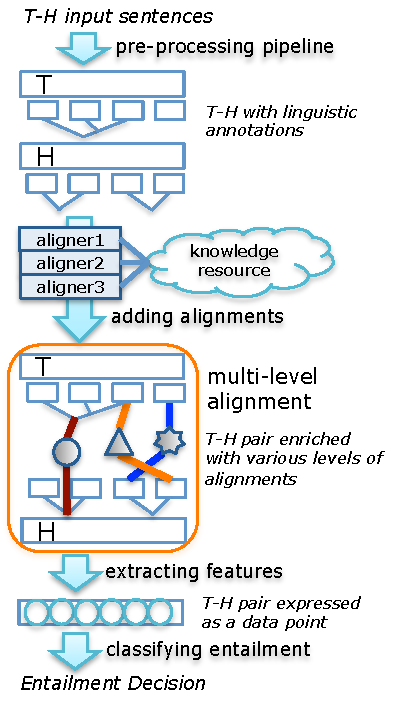
\includegraphics[width=0.9\columnwidth]{figures/figure1.pdf}
  \caption{Dataflow of the proposed approach}
  \label{fig:1}
\end{figure}

First, Text and Hypothesis are pre-processed to establish the
linguistic levels of interest. Then, the annotated T-H pair becomes
the input for various independent aligners, which have access to
knowledge resources and can compute any evidence for or against
entailment that can be represented as a weighted alignment between any
linguistic levels of H and T. Note that this includes many analyses
not normally treated as alignment. Examples include match or
mismatches in negation or modality between parts of T and H, or the
location of where particular inference rules are applicable. The union
of all alignments forms the central data structure, the
{\em Multi-Level Alignment}, shown in the middle of Fig.~1.

The next step is feature extraction. Features can be extracted on the
basis of individal alignments, or from sets of alignments. We assume
that the features form a vector describing the T-H pair, and that the
last step is supervised entailment classification.

\paragraph{Discussion.} The main deviation from Dagan et al.'s
architecture is that we intentionally leave out the step of {\em
  alignment selection} which explicitly selects a single alignment for
each part of H or T, typically the globally most probable one. Our
decision to forgo selection is grounded in our design of Multi-Level
Alignment as a repository that supports coexistence of information
from different sources. This has the following benefits: (a) aligners
become decoupled in that adding a new aligner does not have a direct
impact on the global outcome; (b) alignments produced by different
aligners can have different semantics, e.g. positive (match) or
negative (mismatch); (c) interactions between alignments can still be
captured by defining features in the feature extraction step.

In this manner, Multi-Level Alignment serves as an abstraction layer
that encourages the development of small, self-contained modules that
contribute to TE recognition. Each of these modules consists of two
parts: an aligner, and a set of feature extractors. A priori, each
module can be defined independently; to introduce interactions with
other modules, it should be sufficient to extend the feature
extractors.

The practical benefit for the developer is that even relatively
complex TE systems use a smalls set of well-defined interfaces, which
makes the whole algorithm easy to understand and access, even on the
implementation level. The startup cost is acquaintance with the common
data structure Multi-Level Alignment. We believe that developers are
willing to pay this cost, especially when this provides them with a
platform that already provides multilingual preprocessing and mature
data types.

% % maybe omit --- duplicated in next section 
% Thus, implementing this layer is a very important task for the
% proposed architecture. For this, we borrowed the data structure from
% a TE open-source platform \cite{}. On top of this, we  added {\em
% alignment links} as a generic type that can link any linguistic
% annotation data within the data type. This enabled us to represent
% multi-level alignment layer that can hold any (even future) alignment
% analysis outputs.

% maybe omit --- not many people are interested in SE (software
% engineering) aspects 

\section{Implementation and Evaluation}
\label{sec:impl}
We report a pilot, baseline implementation that tests the potential of 
the proposed architecture. This section first describes the
implementation, then shows the evaluation of the system on two
multi-lingual test set. The implementation, and its source code can 
be accessed from the project homepage \footnote{{URL} anonymized.}.    

\subsection{Pre-processing, knowledge resource, and data
  representation}  
We utilize an open source TE development platform \cite{} as the 
supporting tools for our architecture. The platform provides various   
multilingual pre-processing pipelines, and also knowledge in a
standardized manner for our target languages.
For pre-processing, we have used Maltparser pipelines with TreeTagger
models for all three languages. All knowledge resources (such as
WordNet, VerbOcean, etc) reported in this paper are accessed via the 
platform.    

Another important service that is provided by the platform is the
capability of representing complex data types in a common data
representation. The platform uses UIMA CAS \cite{} as the data
container \cite{}, and defines various annotation types which can be
extended in a coherent manner. This naturally includes linguistic
annotations (such as POS, lemma, parse tree, NER...), but it also
includes the ability to add new meta data type, such as
alignments. This enabled us to define a multilingual multi-level
alignment representation layer, with minimal new data type
definitions. By utilizing those existing modules of a common platform,
we were able to concentrate on the core-algorithm implementations.  

\subsection{The (minimal) aligners}
We used two main aligners for the pilot study. The first aligner is
a generic lexical aligner that works on lemmas via lexical resources,
and the other is a phrase aligner that works on consecutive tokens.  

\paragraph{Lexical aligner} Lexical aligner adds alignment links by
looking up all possible connections between T-H lemmas. If a
relationship is found between two lemmas (one on T and the other on H)
from the given lexical resource, the aligner adds a link between
them. The link has a direction, and has properties of relation name,
and relation strength. Relation name records the type of relation
reported by the lexical resource (such as ``synonym'',
``antonym''). Relation strength is a property that shows the strength
(likelihood) of the relationship, which is often reported by an
automatically built resources such as distributional semantics
tools. The aligner adds all possible links that can be found by the
given lexical resource on the given T-H pair.  

For English, WordNet and VerbOcean were used as the lexical
resources. Italian WordNet was used for Italian, and GermaNet and
German DerivBase \cite{} were used as lexical resources for German. 

\paragraph{Paraphrase aligner} Paraphrase aligner is similar to the
lexical aligner, but what it connects are surface level (tokens),
and it concentrated on more specific resource; the monolingual
paraphrase tables automatically generated by pivot-translation of
Machine Translation tools \cite{}. The alignment links reported by
this aligner has only one relation (paraphrase), but they report
strength of the relation via the translation probability of the
paraphrase. 

In addition to the two aligners, identical lemmas are also aligned
between T-H, without any additional information. In all cases,
aligners report any possible connections they could find, without
regard to existing alignment links.  

Note that the aligners here are minimal, and forms a test-bed, or a
baseline, where additional aligner (analysis) developers can add new
aligners and observe their impacts on TE evaluation. Incorporating
more sophisticated aligners for each language is future work of this
study. Additional aligners such as predicate-compatibility aligner
(for English), and negation aligners (for English and Italian) are
currently in plan.  

\subsection{The (minimal) features} 
We used a set of language independent features in this pilot study. 

The first set is word coverage ratios that measure how much of the
Hypothesis (H) words are covered by local relationship from Text (T)
words. This includes word coverage ratio, and content word coverage
ratio. For the content-word coverage ratio, function words are
filtered based on (language independent) POS classes. The two features 
express general assumption that the more H content covered, the more
likely it is entailment. 

Two other features are Verb coverage, and Proper name coverage
features. Verb-coverage ratio estimates the chance that some
predicate is missed and not covered on Hypothesis. 
Proper name coverage features estimates the chance that the Hypothesis
has a new entity names introduced in H that is not covered by the
components of T. 

Again, the features adopted here can be considered as the base-line
for the approach. Adding new aligners, naturally, requires adding more 
sophisticated features that utilize the added analysis of the new
aligners. We expect that this feature design process is not trivial
and remain to be tested in future work.  

\subsection{Experimental results} 
RTE3 was one of the evaluation workshop for TE community \cite{}. The
evaluation data holds 800 training and 800 testing T-H pairs, and 
later they were translated to both German and Italian. As far as we
know, this is the only RTE evaluation data that is available in
multiple languages with same content. The following table shows the
evaluation result  of the pilot study, marked as {\em proposed},
compared to three other  open-source TE systems that we have tested
with. 

\begin{table}[t!]
\centering
\small
\begin{tabular}{l|ccc}
          &   English   &   German   &   Italian \\
\hline
{\em MultiAlign}&   \textbf{67.0}      &   \textbf{64.5}    &  \textbf{65.4}  \\
BIUTEE        &   \textbf{67.0}      &     -       &     -    \\
TIE           &   65.2       &   63.1    &     -    \\ 
EDITS         &   63.6      &     -       &  62.6  \\ \hline
RTE3 median   &   61.8      &             &          \\

\end{tabular}
\caption{Accuracy evaluation on the RTE3 data set}
\label{table:rte3}
\end{table}

Each of the open source system is configured with their best known
configurations as reported by the developers. The pilot system
supports all three languages, while others supports one (BIUTEE,
English only) or two languages (EDITS, TIE). The pilot system
performed well in all three languages and scored the best among the
tested systems. It ties on the accuracy score with BIUTEE on English,
and it outperforms both EDITS and TIE on English, German and Italian.  

Second task for evaluation is Entailment Graph building. It is an
application task that builds a graph that helps readers to explore
texts in statement levels. Building of the graph requires a TE engine,
and the performance of TE engine is often evaluated with F-1 measure
in this setup. See \cite{} and \cite{} for more information about the
task and data.
The data are from real-world texts of customer interaction domain, and 
they provide large training / test set for TE engine (5300 pairs for
English, 1700 pairs for Italian, etc). Unlike RTE3 data, each data
originated from actual native speakers, and not translated data. Table 
\ref{table:egraph} shows our evaluation results.        

\begin{table}[t!]
\centering
\small
\begin{tabular}{l|ccc}
              &   English    &   Italian   &  German  \\
\hline
{\em MultiAlign}&   69.2     &   \textbf{69.5}    &   \textbf{72.4}  \\
BIUTEE        &   \textbf{71.3}     &     -       &     -     \\
EDITS         &      -       &   65.6    &     -     \\
TIE           &      -       &     -       &   \textbf{72.4}  \\ 
\end{tabular}
\caption{F$_1$ evaluation on entailment graph data}
% balanced, pure-split data.  
\label{table:egraph}
\end{table}

For this task, we ran two systems for each data. One is our pilot
system, and the other is the best engine reported for the data. The
pilot system beats EDITS in Italian data, and closely follows TIE in
German data, while BIUTEE outperforms the pilot system in English
data.   

The two evaluation results show that the pilot system is already
competing with the state-of-the-art open-source TE engines. The fact 
is even more impressive considering that the pilot system is one
system that works on all three languages. We interpret this result as a
positive sign for the future of the proposed architecture, since the
simple baseline for the approach already competes with complex,
mono-lingual TE systems. 

\section{Conclusion (0.5 page)}
This paper introduced a TE architecture that relies on a layer called
{\em multi-level alignments}. The approach closely follows successful  
alignment-based TE architectures, but differs in the sense that the
proposed method encourages having multiple alignments co-existing in 
one common data structure. The approach suggests using this structure
as the ``firewall'' for all analysis, and making TE engine more open
for future improvements.

We reported a baseline, pilot system of this approach, and evaluated
the performance compared to other open-source TE engines. The pilot
system already competes with the state-of-the-art. The system is
extensible, small and robust, and works with multilingual input out of
the box. It is available as open-source, and can be used by 
anyone who requires a multilingual TE engine. We believe that the 
resulting system is easier to access, modify and extend compared to
other open-source TE engines.

%% \section*{Acknowledgments}

%% Do not number the acknowledgment section.
\bibliographystyle{naaclhlt2015}
\bibliography{sem2015_short}

\end{document}
